\documentclass{standalone}
\usepackage{tikz}
\usetikzlibrary{patterns, positioning}

\begin{document}
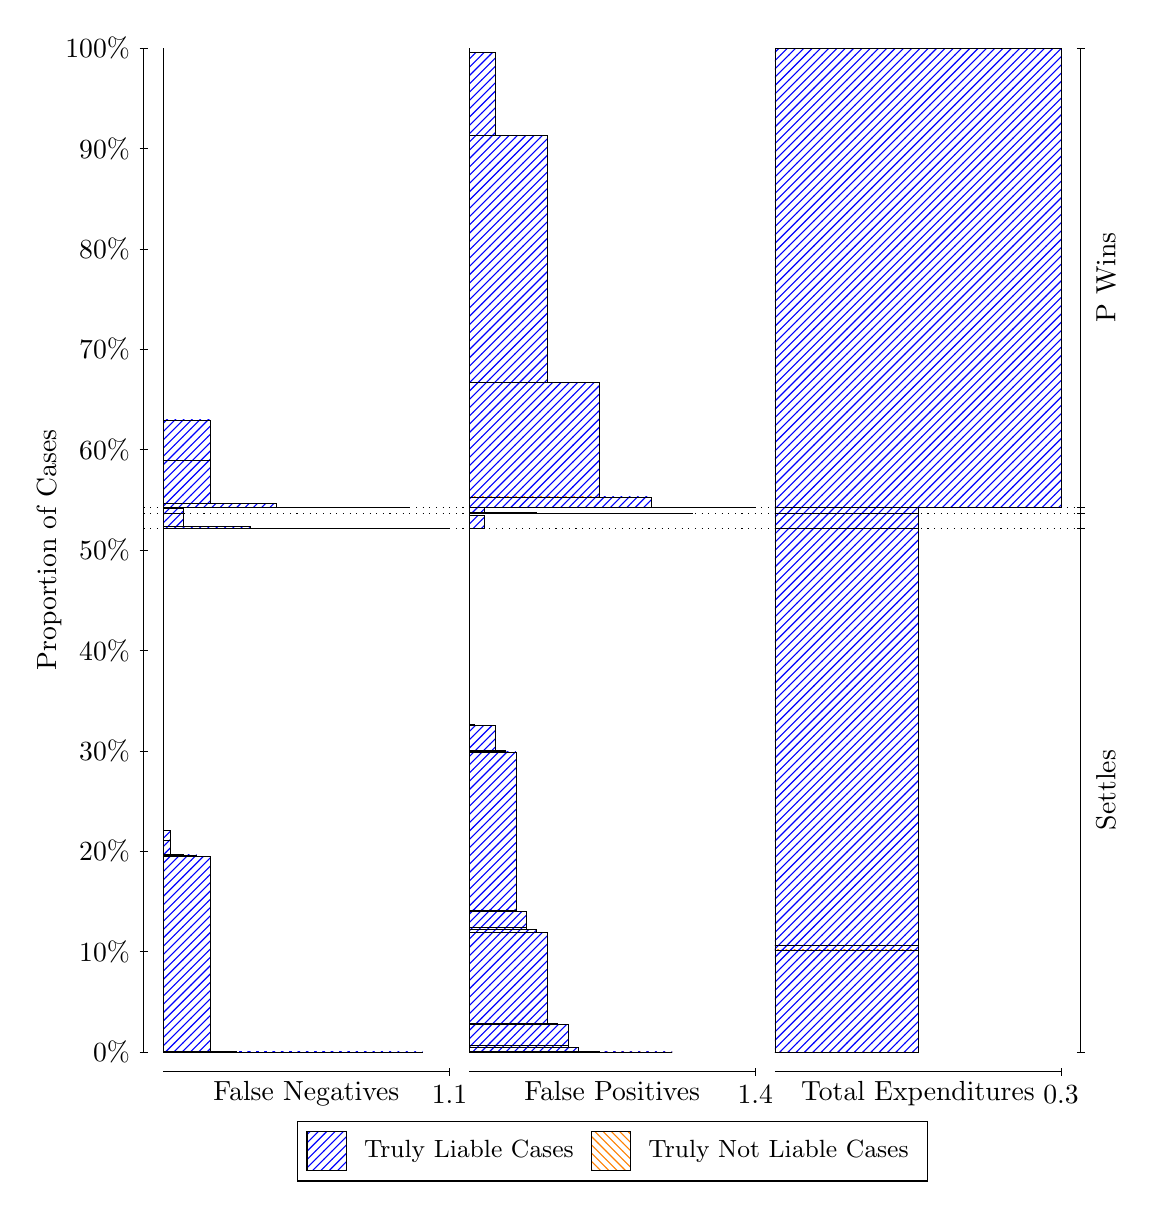
\begin{tikzpicture}
\draw[black, very thin] (1.5,1.75) -- (1.5,14.5);
\node[rotate=90, anchor=center] at (0.3, 8.125) {Proportion of Cases};
\draw[black, very thin] (1.45,1.75) -- (1.55,1.75);
\node[anchor=east] at (1.45, 1.75) {0\%};
\draw[black, very thin] (1.45,3.025) -- (1.55,3.025);
\node[anchor=east] at (1.45, 3.025) {10\%};
\draw[black, very thin] (1.45,4.3) -- (1.55,4.3);
\node[anchor=east] at (1.45, 4.3) {20\%};
\draw[black, very thin] (1.45,5.575) -- (1.55,5.575);
\node[anchor=east] at (1.45, 5.575) {30\%};
\draw[black, very thin] (1.45,6.85) -- (1.55,6.85);
\node[anchor=east] at (1.45, 6.85) {40\%};
\draw[black, very thin] (1.45,8.125) -- (1.55,8.125);
\node[anchor=east] at (1.45, 8.125) {50\%};
\draw[black, very thin] (1.45,9.4) -- (1.55,9.4);
\node[anchor=east] at (1.45, 9.4) {60\%};
\draw[black, very thin] (1.45,10.675) -- (1.55,10.675);
\node[anchor=east] at (1.45, 10.675) {70\%};
\draw[black, very thin] (1.45,11.95) -- (1.55,11.95);
\node[anchor=east] at (1.45, 11.95) {80\%};
\draw[black, very thin] (1.45,13.225) -- (1.55,13.225);
\node[anchor=east] at (1.45, 13.225) {90\%};
\draw[black, very thin] (1.45,14.5) -- (1.55,14.5);
\node[anchor=east] at (1.45, 14.5) {100\%};

\draw[black, very thin] (13.4,1.75) -- (13.4,14.5);
\draw[black, very thin] (13.35,1.75) -- (13.45,1.75);
\node[anchor=west] at (13.35, 1.75) {};
\draw[black, very thin] (13.35,8.4021) -- (13.45,8.4021);
\node[anchor=west] at (13.35, 8.4021) {};
\draw[black, very thin] (13.35,8.5931) -- (13.45,8.5931);
\node[anchor=west] at (13.35, 8.5931) {};
\draw[black, very thin] (13.35,8.6659) -- (13.45,8.6659);
\node[anchor=west] at (13.35, 8.6659) {};
\draw[black, very thin] (13.35,14.5) -- (13.45,14.5);
\node[anchor=west] at (13.35, 14.5) {};

\draw[black, very thin, pattern color=blue, pattern=north east lines] (1.75,1.75) rectangle (5.0453,1.75);
\draw[black, very thin, pattern color=blue, pattern=north east lines] (1.75,1.75) rectangle (4.7074,1.75);
\draw[black, very thin, pattern color=blue, pattern=north east lines] (1.75,1.75) rectangle (4.3694,1.75);
\draw[black, very thin, pattern color=blue, pattern=north east lines] (1.75,1.75) rectangle (4.2004,1.75);
\draw[black, very thin, pattern color=blue, pattern=north east lines] (1.75,1.75) rectangle (4.0314,1.75);
\draw[black, very thin, pattern color=blue, pattern=north east lines] (1.75,1.75) rectangle (3.8624,1.75);
\draw[black, very thin, pattern color=blue, pattern=north east lines] (1.75,1.75) rectangle (3.6934,1.75);
\draw[black, very thin, pattern color=blue, pattern=north east lines] (1.75,1.75) rectangle (3.5244,1.75);
\draw[black, very thin, pattern color=blue, pattern=north east lines] (1.75,1.75) rectangle (3.3554,1.75);
\draw[black, very thin, pattern color=blue, pattern=north east lines] (1.75,1.75) rectangle (3.1864,1.75);
\draw[black, very thin, pattern color=blue, pattern=north east lines] (1.75,1.75) rectangle (3.1864,1.75);
\draw[black, very thin, pattern color=blue, pattern=north east lines] (1.75,1.75) rectangle (3.0174,1.75);
\draw[black, very thin, pattern color=blue, pattern=north east lines] (1.75,1.75) rectangle (2.8484,1.7501);
\draw[black, very thin, pattern color=blue, pattern=north east lines] (1.75,1.7501) rectangle (2.6795,1.7512);
\draw[black, very thin, pattern color=blue, pattern=north east lines] (1.75,1.7512) rectangle (2.6795,1.7527);
\draw[black, very thin, pattern color=blue, pattern=north east lines] (1.75,1.7527) rectangle (2.5105,1.7542);
\draw[black, very thin, pattern color=blue, pattern=north east lines] (1.75,1.7542) rectangle (2.3415,1.7542);
\draw[black, very thin, pattern color=blue, pattern=north east lines] (1.75,1.7542) rectangle (2.3415,1.7544);
\draw[black, very thin, pattern color=blue, pattern=north east lines] (1.75,1.7544) rectangle (2.3415,4.2378);
\draw[black, very thin, pattern color=blue, pattern=north east lines] (1.75,4.2378) rectangle (2.1725,4.2516);
\draw[black, very thin, pattern color=blue, pattern=north east lines] (1.75,4.2516) rectangle (2.0035,4.2563);
\draw[black, very thin, pattern color=blue, pattern=north east lines] (1.75,4.2563) rectangle (1.8345,4.4414);
\draw[black, very thin, pattern color=blue, pattern=north east lines] (1.75,4.4414) rectangle (1.8345,4.5688);
\draw[black, very thin, pattern color=orange, pattern=north west lines] (1.75,4.5688) rectangle (1.75,4.5688);
\draw[black, very thin, pattern color=blue, pattern=north east lines] (1.75,4.5688) rectangle (1.75,8.4021);
\draw[black, very thin, pattern color=blue, pattern=north east lines] (1.75,8.4021) rectangle (5.3833,8.4021);
\draw[black, very thin, pattern color=blue, pattern=north east lines] (1.75,8.4021) rectangle (4.5384,8.4021);
\draw[black, very thin, pattern color=blue, pattern=north east lines] (1.75,8.4021) rectangle (3.6934,8.4023);
\draw[black, very thin, pattern color=blue, pattern=north east lines] (1.75,8.4023) rectangle (2.8484,8.4297);
\draw[black, very thin, pattern color=blue, pattern=north east lines] (1.75,8.4297) rectangle (2.0035,8.5931);
\draw[black, very thin, pattern color=orange, pattern=north west lines] (1.75,8.5931) rectangle (1.75,8.5931);
\draw[black, very thin, pattern color=blue, pattern=north east lines] (1.75,8.5931) rectangle (2.0035,8.6542);
\draw[black, very thin, pattern color=orange, pattern=north west lines] (1.75,8.6542) rectangle (1.75,8.6542);
\draw[black, very thin, pattern color=blue, pattern=north east lines] (1.75,8.6542) rectangle (1.75,8.6659);
\draw[black, very thin, pattern color=blue, pattern=north east lines] (1.75,8.6659) rectangle (4.8764,8.6659);
\draw[black, very thin, pattern color=blue, pattern=north east lines] (1.75,8.6659) rectangle (4.0314,8.6661);
\draw[black, very thin, pattern color=blue, pattern=north east lines] (1.75,8.6661) rectangle (3.1864,8.7185);
\draw[black, very thin, pattern color=blue, pattern=north east lines] (1.75,8.7185) rectangle (2.3415,9.2583);
\draw[black, very thin, pattern color=blue, pattern=north east lines] (1.75,9.2583) rectangle (2.3415,9.7772);
\draw[black, very thin, pattern color=orange, pattern=north west lines] (1.75,9.7772) rectangle (1.75,9.7772);
\draw[black, very thin, pattern color=blue, pattern=north east lines] (1.75,9.7772) rectangle (1.75,14.5);
\draw[black, very thin, pattern color=orange, pattern=north west lines] (5.6333,1.75) rectangle (8.2097,1.75);
\draw[black, very thin, pattern color=blue, pattern=north east lines] (5.6333,1.75) rectangle (8.2097,1.75);
\draw[black, very thin, pattern color=orange, pattern=north west lines] (5.6333,1.75) rectangle (7.9455,1.75);
\draw[black, very thin, pattern color=blue, pattern=north east lines] (5.6333,1.75) rectangle (7.9455,1.75);
\draw[black, very thin, pattern color=orange, pattern=north west lines] (5.6333,1.75) rectangle (7.6812,1.75);
\draw[black, very thin, pattern color=blue, pattern=north east lines] (5.6333,1.75) rectangle (7.6812,1.7502);
\draw[black, very thin, pattern color=blue, pattern=north east lines] (5.6333,1.7502) rectangle (7.5491,1.7518);
\draw[black, very thin, pattern color=orange, pattern=north west lines] (5.6333,1.7518) rectangle (7.417,1.7518);
\draw[black, very thin, pattern color=blue, pattern=north east lines] (5.6333,1.7518) rectangle (7.417,1.752);
\draw[black, very thin, pattern color=blue, pattern=north east lines] (5.6333,1.752) rectangle (7.2848,1.7531);
\draw[black, very thin, pattern color=orange, pattern=north west lines] (5.6333,1.7531) rectangle (7.1527,1.7531);
\draw[black, very thin, pattern color=blue, pattern=north east lines] (5.6333,1.7531) rectangle (7.1527,1.7581);
\draw[black, very thin, pattern color=blue, pattern=north east lines] (5.6333,1.7581) rectangle (7.0206,1.8053);
\draw[black, very thin, pattern color=orange, pattern=north west lines] (5.6333,1.8053) rectangle (6.8885,1.8053);
\draw[black, very thin, pattern color=blue, pattern=north east lines] (5.6333,1.8053) rectangle (6.8885,1.8339);
\draw[black, very thin, pattern color=orange, pattern=north west lines] (5.6333,1.8339) rectangle (6.8885,1.8339);
\draw[black, very thin, pattern color=blue, pattern=north east lines] (5.6333,1.8339) rectangle (6.8885,2.103);
\draw[black, very thin, pattern color=blue, pattern=north east lines] (5.6333,2.103) rectangle (6.7564,2.1161);
\draw[black, very thin, pattern color=orange, pattern=north west lines] (5.6333,2.1161) rectangle (6.6242,2.1161);
\draw[black, very thin, pattern color=blue, pattern=north east lines] (5.6333,2.1161) rectangle (6.6242,3.2684);
\draw[black, very thin, pattern color=blue, pattern=north east lines] (5.6333,3.2684) rectangle (6.4921,3.3041);
\draw[black, very thin, pattern color=orange, pattern=north west lines] (5.6333,3.3041) rectangle (6.36,3.3041);
\draw[black, very thin, pattern color=blue, pattern=north east lines] (5.6333,3.3041) rectangle (6.36,3.3316);
\draw[black, very thin, pattern color=blue, pattern=north east lines] (5.6333,3.3316) rectangle (6.36,3.5307);
\draw[black, very thin, pattern color=blue, pattern=north east lines] (5.6333,3.5307) rectangle (6.2279,3.5554);
\draw[black, very thin, pattern color=blue, pattern=north east lines] (5.6333,3.5554) rectangle (6.2279,5.5611);
\draw[black, very thin, pattern color=orange, pattern=north west lines] (5.6333,5.5611) rectangle (6.0958,5.5611);
\draw[black, very thin, pattern color=blue, pattern=north east lines] (5.6333,5.5611) rectangle (6.0958,5.5719);
\draw[black, very thin, pattern color=blue, pattern=north east lines] (5.6333,5.5719) rectangle (6.0958,5.5833);
\draw[black, very thin, pattern color=blue, pattern=north east lines] (5.6333,5.5833) rectangle (5.9636,5.8958);
\draw[black, very thin, pattern color=blue, pattern=north east lines] (5.6333,5.8958) rectangle (5.8315,5.9005);
\draw[black, very thin, pattern color=blue, pattern=north east lines] (5.6333,5.9005) rectangle (5.6994,5.9055);
\draw[black, very thin, pattern color=blue, pattern=north east lines] (5.6333,5.9055) rectangle (5.6994,5.9144);
\draw[black, very thin, pattern color=blue, pattern=north east lines] (5.6333,5.9144) rectangle (5.6333,8.4021);
\draw[black, very thin, pattern color=orange, pattern=north west lines] (5.6333,8.4021) rectangle (5.8315,8.4021);
\draw[black, very thin, pattern color=blue, pattern=north east lines] (5.6333,8.4021) rectangle (5.8315,8.5656);
\draw[black, very thin, pattern color=blue, pattern=north east lines] (5.6333,8.5656) rectangle (5.6333,8.5931);
\draw[black, very thin, pattern color=orange, pattern=north west lines] (5.6333,8.5931) rectangle (8.4739,8.5931);
\draw[black, very thin, pattern color=blue, pattern=north east lines] (5.6333,8.5931) rectangle (8.4739,8.5931);
\draw[black, very thin, pattern color=blue, pattern=north east lines] (5.6333,8.5931) rectangle (7.8133,8.5931);
\draw[black, very thin, pattern color=blue, pattern=north east lines] (5.6333,8.5931) rectangle (7.1527,8.5932);
\draw[black, very thin, pattern color=blue, pattern=north east lines] (5.6333,8.5932) rectangle (6.4921,8.6049);
\draw[black, very thin, pattern color=blue, pattern=north east lines] (5.6333,8.6049) rectangle (5.8315,8.6659);
\draw[black, very thin, pattern color=orange, pattern=north west lines] (5.6333,8.6659) rectangle (9.2667,8.6659);
\draw[black, very thin, pattern color=blue, pattern=north east lines] (5.6333,8.6659) rectangle (9.2667,8.6659);
\draw[black, very thin, pattern color=orange, pattern=north west lines] (5.6333,8.6659) rectangle (8.6061,8.6659);
\draw[black, very thin, pattern color=blue, pattern=north east lines] (5.6333,8.6659) rectangle (8.6061,8.6676);
\draw[black, very thin, pattern color=orange, pattern=north west lines] (5.6333,8.6676) rectangle (7.9455,8.6676);
\draw[black, very thin, pattern color=blue, pattern=north east lines] (5.6333,8.6676) rectangle (7.9455,8.7998);
\draw[black, very thin, pattern color=orange, pattern=north west lines] (5.6333,8.7998) rectangle (7.2848,8.7998);
\draw[black, very thin, pattern color=blue, pattern=north east lines] (5.6333,8.7998) rectangle (7.2848,10.254);
\draw[black, very thin, pattern color=orange, pattern=north west lines] (5.6333,10.254) rectangle (6.6242,10.254);
\draw[black, very thin, pattern color=blue, pattern=north east lines] (5.6333,10.254) rectangle (6.6242,13.389);
\draw[black, very thin, pattern color=blue, pattern=north east lines] (5.6333,13.389) rectangle (5.9636,14.447);
\draw[black, very thin, pattern color=blue, pattern=north east lines] (5.6333,14.447) rectangle (5.6333,14.5);
\draw[black, very thin, pattern color=orange, pattern=north west lines] (9.5167,1.75) rectangle (11.333,1.75);
\draw[black, very thin, pattern color=blue, pattern=north east lines] (9.5167,1.75) rectangle (11.333,3.0472);
\draw[black, very thin, pattern color=orange, pattern=north west lines] (9.5167,3.0472) rectangle (11.333,3.0472);
\draw[black, very thin, pattern color=blue, pattern=north east lines] (9.5167,3.0472) rectangle (11.333,3.1049);
\draw[black, very thin, pattern color=orange, pattern=north west lines] (9.5167,3.1049) rectangle (11.333,3.1049);
\draw[black, very thin, pattern color=blue, pattern=north east lines] (9.5167,3.1049) rectangle (11.333,8.4021);
\draw[black, very thin, pattern color=orange, pattern=north west lines] (9.5167,8.4021) rectangle (11.333,8.4021);
\draw[black, very thin, pattern color=blue, pattern=north east lines] (9.5167,8.4021) rectangle (11.333,8.5931);
\draw[black, very thin, pattern color=orange, pattern=north west lines] (9.5167,8.5931) rectangle (11.333,8.5931);
\draw[black, very thin, pattern color=blue, pattern=north east lines] (9.5167,8.5931) rectangle (11.333,8.6659);
\draw[black, very thin, pattern color=orange, pattern=north west lines] (9.5167,8.6659) rectangle (13.15,8.6659);
\draw[black, very thin, pattern color=blue, pattern=north east lines] (9.5167,8.6659) rectangle (13.15,14.5);
\draw[black, dotted] (1.5,8.4021) -- (13.4,8.4021);
\draw[black, dotted] (1.5,8.5931) -- (13.4,8.5931);
\draw[black, dotted] (1.5,8.6659) -- (13.4,8.6659);
\draw[black, very thin] (1.75,1.5) -- (5.3833,1.5);
\node[anchor=north] at (3.5667, 1.5) {False Negatives};
\draw[black, very thin] (5.3833,1.45) -- (5.3833,1.55);
\node[anchor=north] at (5.3833, 1.45) {1.1};

\draw[black, very thin] (5.6333,1.5) -- (9.2667,1.5);
\node[anchor=north] at (7.45, 1.5) {False Positives};
\draw[black, very thin] (9.2667,1.45) -- (9.2667,1.55);
\node[anchor=north] at (9.2667, 1.45) {1.4};

\draw[black, very thin] (9.5167,1.5) -- (13.15,1.5);
\node[anchor=north] at (11.333, 1.5) {Total Expenditures};
\draw[black, very thin] (13.15,1.45) -- (13.15,1.55);
\node[anchor=north] at (13.15, 1.45) {0.3};

\node[black, centered, rotate=90] at (13.72, 5.0761) {Settles};


\node[black, centered, rotate=90] at (13.72, 11.583) {P Wins};

\draw (7.449999999999999,1.5) node[draw=none] (baseCoordinate) {};
\begin{scope}[align=center]
        \matrix[scale=0.5, draw=black, below=0.5cm of baseCoordinate, nodes={draw}, column sep=0.1cm]{
            \node[rectangle, draw, minimum width=0.5cm, minimum height=0.5cm, pattern=north east lines, pattern color=blue] {}; &
            \node[draw=none, font=\small] (B) {Truly Liable Cases}; &
            \node[rectangle, draw, minimum width=0.5cm, minimum height=0.5cm, pattern=north west lines, pattern color=orange] {}; &
            \node[draw=none, font=\small] (B) {Truly Not Liable Cases}; \\
            };
\end{scope}

\end{tikzpicture}
\end{document}